\documentclass[a4paper,12pt]{article}
\usepackage[spanish]{babel}
\usepackage[utf8]{inputenc}
\usepackage{booktabs}
\usepackage{dirtytalk}
\usepackage{graphicx}
\usepackage{makecell}

\begin{document}

\title{\Large Instituto Politécnico Nacional\\Escuela Superior de Cómputo\\Redes de Computadoras\\Tarea 2: Organizaciones\\Alumno: Meza Zamora Abraham Manuel}
\date{}
\maketitle

\section{ICANN}
La Corporación de Internet para la Asignación de Nombres y Números, es una organización que opera a nivel internacional y es la responsable de asignar las direcciones del protocolo IP, de los identificadores de protocolo, de las funciones de gestión del sistema de dominio y de la administración del sistema de servidores raíz.

En la actualidad, la ICANN está formalmente organizada como una corporación sin fines de lucro y de utilidad pública.

ICANN coordina la administración de los elementos técnicos del Sistema de Nombres de Dominio (DNS) para garantizar la resolución unívoca de los nombres, de esta manera los usuarios puedan encontrar todas las direcciones IP sin ser repetidas.

En la actualidad hay tres organizaciones de apoyo: 
\begin{itemize}
\item GNSO (Generic Names Supporting Organization) se ocupa de la formulación de políticas sobre
dominios genéricos de nivel superior.
\item ccNSO (Country Code Names Supporting Organization) se ocupa de la elaboración de políticas relativas a códigos de países en dominios de nivel superior.
\item ASO (Address Supporting Organization) se ocupa de la formulación de políticas en direcciones IP.
\end{itemize}

ICANN periódicamente sostiene reuniones públicas de rotación entre los continentes para fomentar la participación mundial en sus procesos. Los críticos argumentan que los lugares de estas reuniones se encuentran a menudo en los países con menor uso de Internet. 

ICANN sigue en el mismo edificio donde se creó, que es una oficina del Instituto de Ciencias de la Información en la Universidad del Sur de California.

\section{IANA}
Es la entidad que supervisa la asignación global de las direcciones de IP, sistemas autónomos, servidores raíz de nombres de dominio DNS y otros recursos relativos a los protocolos de Internet. Actualmente es un departamento operado por ICANN.

\section{Registros regionales de Internet}
Es una organización que supervisa la asignación y el registro de recursos de números de Internet dentro de una región particular del mundo.

Actualmente hay 5 RIR en funcionamiento.
\begin{itemize}
\item American Registry for Internet Numbers (ARIN) para América Anglosajona.
\item RIPE Network Coordination Centre (RIPE NCC).
\item para Europa, el Oriente Medio y Asia Central.
\item Asia-Pacific Network Information Centre (APNIC) para Asia y la Región Pacífica.
\item Latin American and Caribbean Internet Address Registry (LACNIC) para América Latina y el Caribe.
\item AfricanNetworkInformationCentre(AfriNIC) para África.
\end{itemize}

Todos los dispositivos conectados a una red IP necesitan tener una dirección IP. Las direcciones IP y los números de sistema autónomo son recursos finitos. Esto significa que algún día se agotarán. Es necesario que haya un manejo neutral y efectivo de estos recursos para asegurar la distribución justa e igualitaria así como para prevenir el acaparamiento.

La Corporación de Internet para la Asignación de Nombres y Números (ICANN) delega los recursos de Internet a los RIR, y a su vez los RIR siguen sus políticas regionales para una posterior subdelegación de recursos a sus clientes, que incluyen proveedores de servicios de Internet (ISP) y organizaciones para uso propio.
\section{ISP}
El \textit{proveedor de servicios de Internet} es la empresa que brinda conexión a Internet a sus clientes. Un ISP conecta a sus usuarios a Internet a través de diferentes tecnologías como DSL, cable módem, GSM, dial-up, etcétera.

Originalmente, para acceder a Internet se necesitaba una cuenta universitaria o de alguna agencia del gobierno; que necesariamente tenía que estar autorizada. Internet comenzó a aceptar tráfico comercial a principios de la década de 1990, pero era demasiado limitada y en una cantidad mínima en comparación con la actualidad. 

En 1995 el MIT y AT\&T comenzaron a cobrar a los usuarios una renta mensual alrededor de los 20 \$ USD. A los negocios se les aumentaba esta tarifa, ya que disponían de una conexión más rápida y fiable.

Cuando Internet evolucionó repentinamente, los ISP fueron desafiados drásticamente a actualizar su infraestructura, tecnologías y a incrementar sus puntos de acceso.

Los accesos se mejoraron, así que el uso de Internet creció exponencialmente, llevando a bajar los precios mensuales de los ISP, aunque variando por cada país. En países con pocos ISP, los cuales tenían un gran monopolio, se solía cobrar más que en lugares donde existe una situación de competencia real, la cual previene que las compañías suban demasiado.
\section{Who is}

es un protocolo TCP basado en petición/respuesta que se utiliza para efectuar consultas en una base de datos que permite determinar el propietario de un nombre de dominio o una dirección IP en Internet. Las consultas WHOIS se han realizado tradicionalmente usando una interfaz de línea de comandos, pero actualmente existen multitud de páginas web que permiten realizar estas consultas. Estas páginas siguen dependiendo internamente del protocolo WHOIS para conectar a un servidor WHOIS y hacer las peticiones. Los clientes de línea de comandos siguen siendo muy usados por los administradores de sistemas.

\begin{figure}[h]
\centering
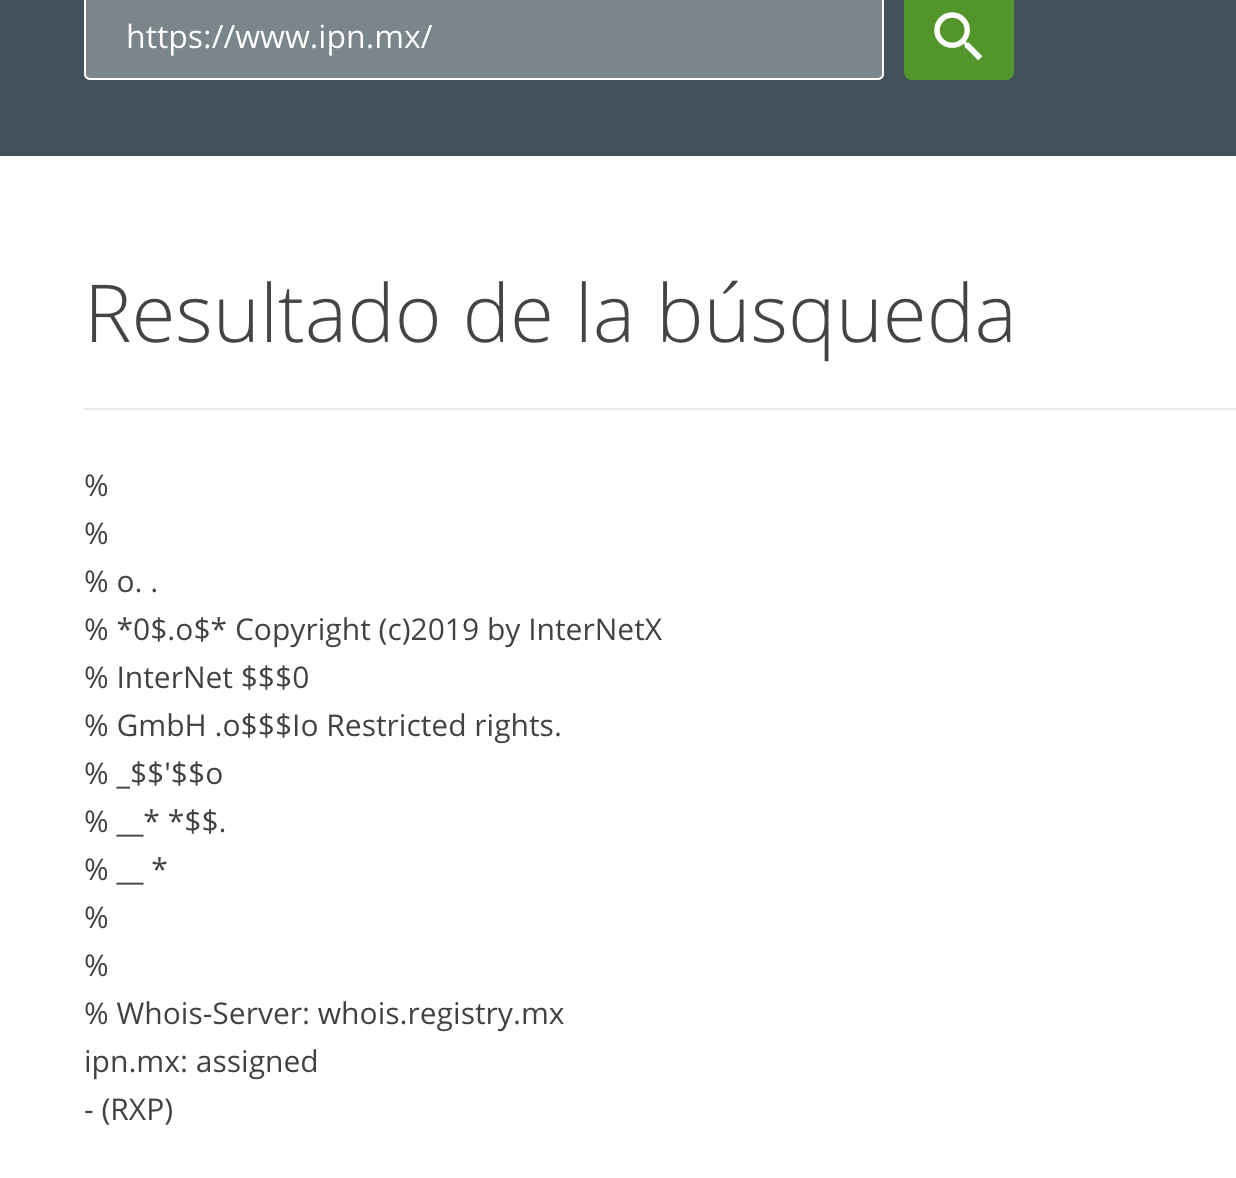
\includegraphics[width=0.60\textwidth]{figuno}
\caption{Who is de la página de ESCOM.}
\end{figure}

\begin{thebibliography}{12}
\bibitem{uno} 
"Internet Assigned Numbers Authority" (https://www.iana.org/). Public Technical Identifiers. Retrieved 17 December 2011.

\bibitem{dos}
Comisión Nacional de Comunicaciones. «CNC. Tipos de Conexión (http://www.cnc.gob.ar/infotecnica/radioaficionad os/raf.asp?valor1=senaldistintiva\&valor2=DESC\&busq=\&offset=5750). Consultado el 21 de octubre de 2014.

\bibitem{tres}
 http://www.whoisdominio.com (http://www.whoisdominio.com)
 
\end{thebibliography}

\end{document}